% Section content template for individual Educative lessons
% This file contains the actual content for a specific section
% Generated from Educative API section content

% Section: Getting Ready: Elevator System
% Section ID: 5598619459911680
% Section Slug: getting-ready-elevator-system
% Generated: 2025-12-11T14:04:33.296489

\subsection{Problem definition}\label{KfyitG1dioESlbYIcgWus-1}
\\
\textbf{Elevators} are essential in multi-story buildings, enabling the efficient movement of people and goods. A typical system includes one or more elevator cars that respond to user requests from call buttons on each floor and destination selections inside the car.
\\
To ensure efficiency and safety, an elevator system must handle requests intelligently, minimize passenger wait times, respect car capacity, and support centralized and decentralized control of multiple cars. The system must also manage concurrent requests, optimize car movements, and provide real-time feedback through displays inside and outside the cars.
\\
Robust safety protocols are critical: in emergencies like power failures or fire alarms, the system may need to ignore inputs and keep doors closed until operation is safe. Handling such scenarios correctly is essential for user protection and reliable operation.
\\
In this LLD interview case study, you'll focus on:

\begin{itemize}
\item
\protect\phantomsection\label{7ysMHeCvKrPak4seUScw_}
\textbf{Multiple elevators coordination:} Distributing requests among cars and managing their interaction.
\item
\protect\phantomsection\label{gDMPFNvvlQnki9c6CMGO5}
\textbf{Request scheduling:} Prioritizing and queuing floor requests.
\item
\protect\phantomsection\label{PIkZqKw0tB13HTKvTC4DV}
\textbf{Capacity management:} Preventing overloading.
\item
\protect\phantomsection\label{vN0qxhn22V2MbQzqE1rPc}
\textbf{Real-time updates:} Showing current floor, direction, and occupancy.
\item
\protect\phantomsection\label{zpGay_46QWSCE-NuJpBwI}
\textbf{Safety and fault tolerance:} Managing emergencies and critical faults.
\item
\protect\phantomsection\label{9os1a8w-empbO-QDjczNb}
\textbf{User experience:} Minimizing wait times, supporting up/down requests, and providing clear information.
\end{itemize}
\\
This elevator system case study requires you to design a scalable, reliable, and user-friendly system that can be adapted to different building sizes and requirements.

\begin{figure}[htbp]
 \centering
 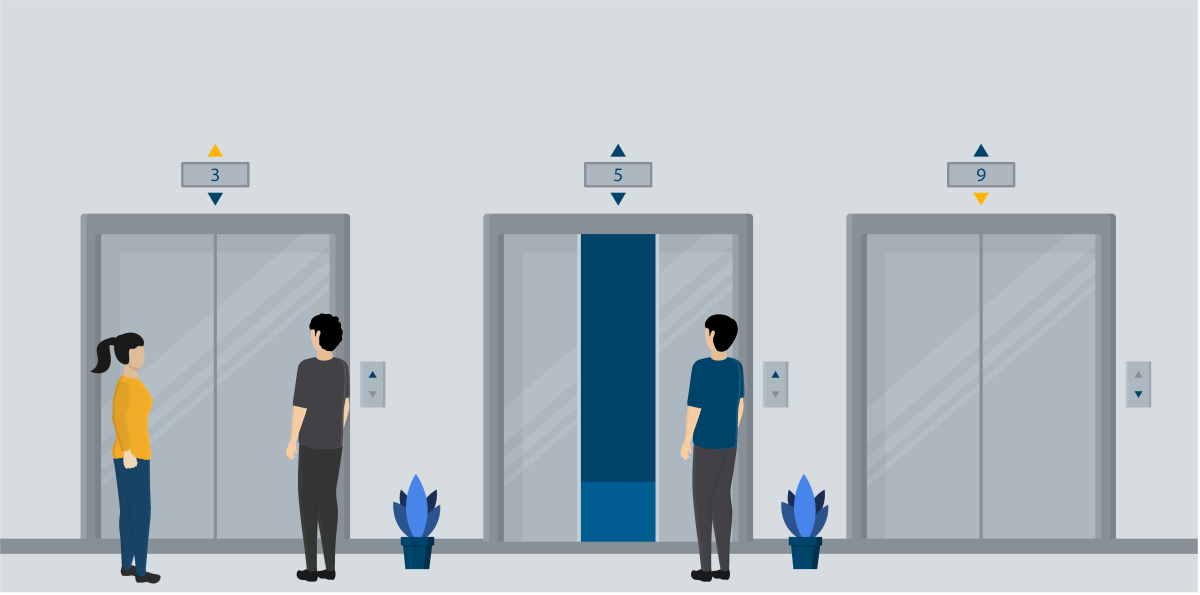
\includegraphics[width=0.5\textwidth]{Images/chapter_8/section_5598619459911680/6293528759238656.png}
 \caption{The elevator system}
\end{figure}

\subsection{Expectations from the interviewee}\label{KfyitG1dioESlbYIcgWus-2}
\\
Numerous components are present in a typical elevator system, each with specific constraints and requirements. Interviewers look for your ability to break down and design the system, anticipate real-world scenarios, and identify components and interactions. Typical areas of exploration include:

\subsubsection{Multiple elevators}\label{0z6y1u1KiL-KKltuRwDPM}
\\
You can also ask the interviewer whether the system should handle multiple elevators or just a single one. For this, you can ask the following questions:

\begin{enumerate}
\item
\protect\phantomsection\label{uSpyhN4hj9jEDjxuesdv1}
Can there be multiple elevator cars in the building?
\item
\protect\phantomsection\label{K9q_rPUiby4Js7frX0Rvw}
How could a one-elevator system differ from a multi-elevator system regarding user wait time and running cost?
\end{enumerate}

\subsubsection{Display}\label{BcvDHPFMM9f8gC6pGi363}
\\
You may want to ask the interviewer about the display of the elevator system:

\begin{enumerate}
\item
\protect\phantomsection\label{h0dSAi64ZQkucPE6IXcW5}
How will users request elevators (call panels on each floor, selection panels inside cars)?
\item
\protect\phantomsection\label{XFwWz5jJH1kzr8WY2A9Eg}
What information is shown on displays inside and outside the elevator cars (current floor, direction, occupied status)?
\item
\protect\phantomsection\label{gIuzVfL8HOGCVwqTyf8-v}
How do you keep users informed of the system state and updates?
\end{enumerate}

\subsubsection{Optimization}\label{bUI00MJsoCldRJEfF3gOc}
\\
An interviewer would expect you to ask questions about optimizing the elevator system regarding wait time, maintenance, throughput, etc. You can ask questions like:

\begin{enumerate}
\item
\protect\phantomsection\label{CCV6iyNLbwSDKfwIE1iy-}
What strategies can minimize passenger wait times and unnecessary car movements?
\item
\protect\phantomsection\label{HHccu8hRUrVhLMarsjDO1}
How does the system handle peak hours and concurrent requests?
\item
\protect\phantomsection\label{joo42wPU-SUbw1hUxsu6E}
How do you optimize user experience and operational efficiency (energy use, maintenance)?
\end{enumerate}

\subsubsection{Reliablity and safety}\label{f1Wunzz89vPHSOpE-Jt0P}
\\
You may want to ask the interviewer about the safety and reliability of the elevator system:

\begin{enumerate}
\item
\protect\phantomsection\label{XN95nzHjDZqjHBXDVJX48}
How does the system respond to faults, emergencies, or overloaded conditions?
\item
\protect\phantomsection\label{-W4j5HgAl7MNaZF1sYSfF}
What features ensure passenger safety at all times?
\end{enumerate}

\subsection{Design approach}\label{lcLaxF82jBzm0oNdVfG7K}
\\
In this case study, we`ll take a bottom-up design approach:

\begin{enumerate}
\item
\protect\phantomsection\label{P9l4Z-e65pwr1nrJHE1EK}
\textbf{Start small:} Identify and design the smallest building blocks of the system, such as buttons, doors, and displays.
\item
\protect\phantomsection\label{N8NXqdnxE8TB77BgUiLqc}
\textbf{Compose larger components:} Use these small components to assemble larger modules, such as the elevator car, request panels, and floor subsystems.
\item
\protect\phantomsection\label{kTUqqHi9y5usyEqw_kOSg}
\textbf{Integrate into the full system:} Combine these pieces to design a building's complete elevator control system.
\item
\protect\phantomsection\label{CuIJZROnYKFfOawuwMVK6}
\textbf{Iterative refinement:} At each stage, consider interactions, constraints, and edge cases; iterate and refine based on system requirements.
\end{enumerate}
\\
This approach helps ensure the design is modular, extensible, and robust, and makes it easier to adapt the solution for varying building types and requirements.

\subsection{Design pattern~}\label{6tiJ6hFlAnJ2c_EuVhEuw}
\\
During an interview, discussing the design patterns that an elevator system falls under is always a good practice. Stating the design patterns gives the interviewer a positive impression and shows that the interviewee is well-versed in the advanced concepts of object-oriented design.
\\
Try to answer the following question. If you are not familiar with design patterns, don't worry! You can learn about them by asking questions like, ``Define design patterns.''

\textbf{Question:}

Which design pattern(s) should be used to design an elevator system? Please explain your choice(s).

Let's explore the requirements of the elevator system in the next lesson.

% End of section content